\documentclass[12pt,twoside,draft]{book}
\usepackage{../../thesis}
\graphicspath{ {../../images/} }
\usepackage{tikz}
\usetikzlibrary{arrows,positioning} 
\tikzset{
    %Define standard arrow tip
    >=stealth',
    %Define style for boxes
    punkt/.style={
           rectangle,
           rounded corners,
           draw=black, very thick,
           text width=6.5em,
           minimum height=2em,
           text centered},
    % Define arrow style
    imply/.style={
           ->,
           thick,
           shorten <=2pt,
           shorten >=2pt,},
    both/.style={
           <->,
           thick,
           shorten <=2pt,
           shorten >=2pt,},
    induced/.style={
           dotted,
           ->,
           thick,
           shorten <=2pt,
           shorten >=2pt,},
}

\makeindex
\begin{document}
\chapter{Comparisons of Definitions of Chaos}
We have seen four definitions 
\begin{enumerate}[(i)]
  \item Positive topological entropy
  \item Devaney
  \item Block-Coppel
  \item Li-Yorke
\end{enumerate}
and their variants
\begin{enumerate}[(i)]
  \item Wiggins's (similar to Devaney)
  \item Martelli (equivalent to Wiggins's in $\R^n$)
  \item Marotto (implies Li-Yorke. Requires differentiability)
\end{enumerate}
In this chapter, we discuss the relations between the first four definitions.
(Why omit the latter three?)
Throughout this chapter, we consider the dynamical system $(X,F)$, where $X$ is a metric space, and $F$ is a continuous mapping.
Specifically, we consider the case where $X$ is a compact interval, compact subset of $\R^n$, and compact metric space.


\section{Compact Interval}
Let $I \subseteq \R$ be a compact interval.
In this section, we consider the case where $X = I$.
As it turns out, Devaney's, Block-Coppel's, and positive topological entropy are equivalent conditions, and Li-Yorke's chaos is a weaker condition.
\begin{figure}[ht]
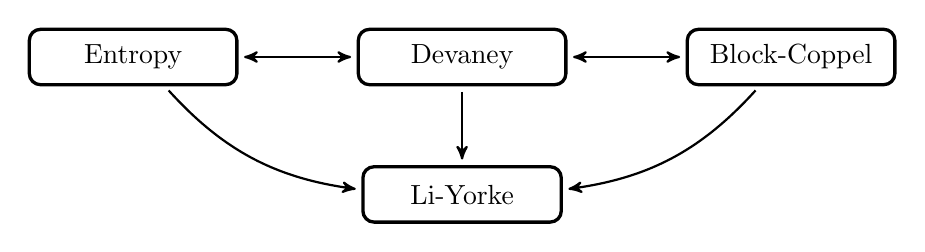
\begin{tikzpicture}[node distance=1cm, auto,]
 %nodes
 \node[punkt] (ly) {Li-Yorke};
 \node[punkt, inner sep=5pt,above=1.0cm of ly] (dev) {Devaney};
 \node[punkt, inner sep=5pt,right=1.5cm of dev] (bc) {Block-Coppel};
 \node[punkt, inner sep=5pt,left=1.5cm of dev] (entropy) {Entropy};
 %edges
 \draw[imply] (dev) to node {} (ly); 
 \draw[imply] (entropy) to[bend right=20] node {} (ly); 
 \draw[imply] (bc) to[bend left=20] node {} (ly); 
 \draw[both] (dev) to node {} (entropy); 
 \draw[both] (dev) to node {} (bc); 
 \end{tikzpicture}
\caption{Relations between definitions for a compact interval.}
\end{figure}

\citet{aulbach} discuss the equivalence between Devaney's and Block-Coppel's definitions.
\begin{theorem}
  \citep{aulbach}
  $(I,F)$ is chaotic in Devaney's sense if and only if it is chaotic in Block-Coppel's sense.
  \label{devaney-blockcoppel}
\end{theorem}

\citet{forti} mentions that the following can be proved using the method in \citet{omegachaos}. (Questionable. See Balibrea, Snoha)
\begin{theorem}
  $(I,F)$ is chaotic in the sense of Devaney if and only if it has positive topological entropy.
  \label{thm:devaney-entropy}
\end{theorem}

As a side note, let us mentions that, on a compact interval, Devaney's and Wiggins's definitions are equivalent.
\begin{theorem}
   $(I,F)$ is chaotic in the sense of Devaney if and only if it is chaotic in the sense of Wiggins.
  \label{thm:devaney-wiggins}
  \begin{proof}
    We mentioned that dense periodic orbits and topological transitivity imply sensitive dependence on initial conditions in a compact metric space.
    The same author, \citet{silverman}, has also shown that on a compact interval, topological transitivity implies the existence of dense periodic orbits and sensitive dependence on initial conditions.
  \end{proof}
\end{theorem}

\begin{theorem}
  \citep{blockcoppel}
  If $(I,F)$ is chaotic in Block-Coppel's sense, then it is chaotic in Li-Yorke's sense.
  \label{thm:devaney-liyorke}
  \begin{proof}
    See \citet{blockcoppel} (VI; Proposition 27).
  \end{proof}
\end{theorem}

\citet{aulbach} and \citet{smital} show that Li-Yorke's chaos does not imply Block-Coppel and positive topological entropy, respectively.
\begin{theorem}
  \citep{aulbach, smital}
  Chaos in Li-Yorke is not a sufficient condition for chaos in Block-Coppel's sense and does not imply positive topological entropy.
  \label{thm:counterexample1}
\end{theorem}

In summary, Devaney's, Block-Coppel's, and positive topological entropy definitions are equivalent on a compact interval.
Each of the three equivalent definitions imply chaos in Li-Yorke's sense, but Li-Yorke's definition does not imply others.


\section{Compact Metric Space}

\begin{figure}[ht]
  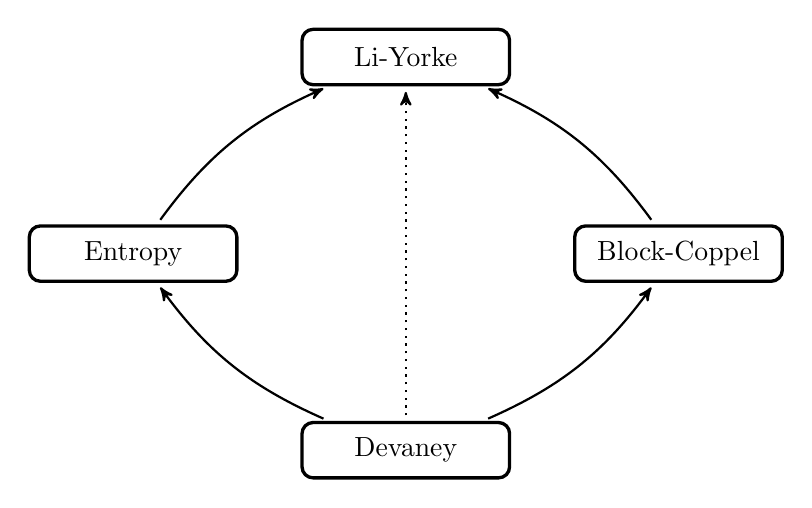
\begin{tikzpicture}[node distance=1cm, auto,]
 %nodes
    \node[] (dummy) {};
    \node[punkt, inner sep=5pt,above=2.0cm of dummy] (ly) {Li-Yorke};
    \node[punkt, inner sep=5pt,below=2.0cm of dummy] (dev) {Devaney};
    \node[punkt, inner sep=5pt,right=2.0cm of dummy] (bc) {Block-Coppel};
    \node[punkt, inner sep=5pt,left=2.0cm of dummy] (entropy) {Entropy};
 %edges
    \draw[induced] (dev) to node {} (ly); 
    \draw[imply] (entropy) to[bend left=15] node {} (ly); 
    \draw[imply] (bc) to[bend right=15] node {} (ly); 
    \draw[imply] (dev) to[bend left=15] node {} (entropy); 
    \draw[imply] (dev) to[bend right=15] node {} (bc); 
  \end{tikzpicture}
  \caption{Relations between definitions for a compact interval.}
\end{figure}

\citet{blanchard} has shown that posivite topological entropy implies chaos in Li-Yorke's sense .
\begin{theorem}
  If $(X,F)$ has positive topological entropy, then it is chaotic in Li-Yorke's sense.
  \label{thm:entropy-liyorke}
\end{theorem}

There exists a system that is topologically transitive and sensitive to initial conditions, but not chaotic in Li-Yorke's sense.
\begin{theorem}
  \citep{blanchard}
  Chaos in Wiggins's sense is not a sufficient condition for chaos in Li-Yorke's sense.  
  \begin{proof}
    Irrational Rotation is topologically transitive, and sensitive to initial conditions.
    However, it does not have a Li-Yorke pair. 
  \end{proof}
\end{theorem}

\citet{aulbach} has shown that Li-Yorke's and Block-Coppel's definitions are weaker than Devaney's definition.
\begin{theorem}
  \citep{aulbach} 
  The adding machine is chaotic in Li-Yorke's sense \textbf{and} in Block-Coppel's sense.
  However, the system is not chaotic in Devaney's sense.
  \begin{proof}
    (Adding machine example)
  \end{proof}
\end{theorem}

In summary,

\bibliographystyle{../../bibliography/pjgsm}
\bibliography{../../bibliography/thesis}

\printindex
\end{document}

